
\vfill
\section{Workflow}

\begin{figure*}[h]
\centering
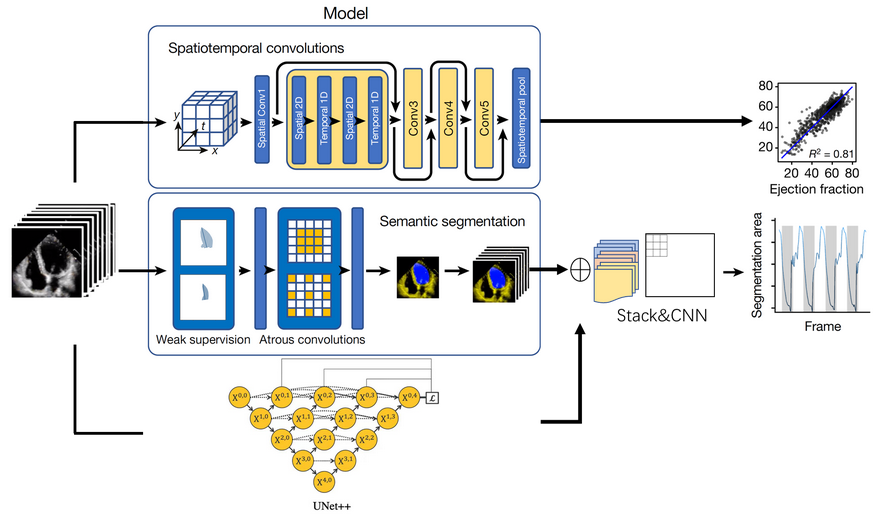
\includegraphics[width=0.9\textwidth]{workflow}
\caption{EchoNet-Dynamic architecture}
\label{EchoNet-Dynamic}
\end{figure*}

EchoNet-Dynamic has three key components(Figure \ref{EchoNet-Dynamic}). First, it constructed a CNN model with atrous convolutions for frame-level semantic segmentation of the left ventricle. The technique of atrous convolutions enables the model to capture larger patterns and has previously been shown to perform well on non-medical imaging datasets.The standard human clinical workflow for estimating the ejection fraction requires manual segmentation of the left ventricle during end systole and end diastole. We generalize these labels in a weak supervision approach with atrous convolutions to generate frame-level semantic segmentation throughout the cardiac cycle in a 1:1 pairing with frames from the original video. The automatic segmentation is used to identify ventricular contractions and provides a clinician-interpretable intermediary that mimics the clinical workflow.

Second, it trained a CNN model with residual connections and spatiotemporal convolutions across frames to predict the ejection fraction. In contrast to previous CNN architectures for machine learning of medical images, our approach integrates spatial as well as temporal information in our network convolutions. Spatiotemporal convolutions,which incorporate spatial information in two dimensions as well as temporal information in the third dimension, have previously been used in non-medical video-classification tasks. However, this approach has not previously been used for medical data given the relative scarcity of labelled medical videos.

In EchoNet-Dynamic's architecture, integrating UNet++ with a three-layer design alongside DeepLabV3 is aimed to enhance model performance. UNet++ optimizes semantic segmentation through dense skip connections, capturing more contextual information and reducing information loss. By concatenating this with DeepLabV3, we aim to combine their segmentation strengths, especially in detailing left ventricle structures, to improve ejection fraction estimation accuracy. This integration seeks to enrich contextual understanding crucial for analyzing cardiac function, thereby aiming to optimize EchoNet-Dynamic's reliability in cardiac function assessment.

Finally, it makes video-level predictions of the ejection fraction for beat-to-beat estimations of cardiac function. Given that variation in cardiac function can be caused by changes in loading conditions as well as heart rate in a variety of cardiac conditions, it is recommended to perform estimations of the ejection fraction for up to five cardiac cycles; however, this is not always done in clinical practice given the tedious and laborious nature of the calculation. Our model identifies each cardiac cycle, generates a clip of 32 frames and averages clip-level estimates of the ejection fraction for each beat as test-time augmentation. EchoNet-Dynamic was developed using 10,030 apical four-chamber echocardiogram videos obtained during the course of routine clinical practice at Stanford Medicine.
